\section{Durchführung und Versuchsaufbau}

    \subsection{Zeitkonstante}

        \noindent Im ersten Versuchsteil soll die Zeitkonste $RC$ gemessen werden. In dieser Versuchsreihe wird an dem Oszilloskop die Schaltung nach 
        Abbildung(\ref{img:Zeit}) aufgebaut. Hier wird nun das Aufladen oder Entladen eines Kondensator der Kapazität $C$ über einen Widerstand 
        $R$ betrachtet. Dazu wird eine Rechteckspannung angelegt und die Achsenskallierung so angepasst, dass entweder der Aufladevorgang oder der 
        Entladevorgang komplett abzulesen ist. Nun können 30 Wertepaare für $U_{\text{C}}(t)$ abgelesen werden. 

        \begin{figure}
            \centering
            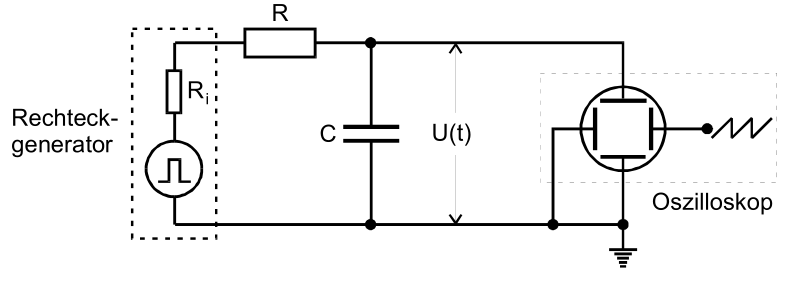
\includegraphics[width=0.7\textwidth]{latex/images/Zeitkonstante.PNG}
            \caption{Schaltbild zur Bestimmung eines RC-Kreis durch Beobachtung des Auf- oder Entladevorganges des Kondensators.\protect \cite{V353}.}
            \label{img:Zeit}
        \end{figure}

    \subsection{Amplitude der Kondensatorspannung in Abhängigkeit der Frequenz}

        \noindent Die zweite Messreihe wird mit dem Schaltbild aus Abbildung(\ref{img:Zeit}) durchgeführt. Hier wird ein Millivoltmeter genutzt 
        um die Kondensatorspannung A in Abhängigkeit von der Frequenz zu messen. Die Frequenz soll dazu über 3 Zehnerpotenz variiert werden. Der 
        Widerstand aus der Schaltung wird mit einem digitalen Ohmmeter vermessen. 

        \begin{figure}
            \centering
            \includegraphics[width=0.7\textwidth]{latex/images/Frequenzabhängigkeit.PNG}
            \caption{Schaltbild zur Bestimmung der Frequenzabhängigkeit der Kondensatorspannungsamplitude A in einem RC-Kreis.\protect \cite{V353}.}
            \label{img:Zeit}
        \end{figure}

    \subsection{Phasenverschiebung in Abhängigkeit der Frequenz}
        \begin{figure}[H]
            \centering
            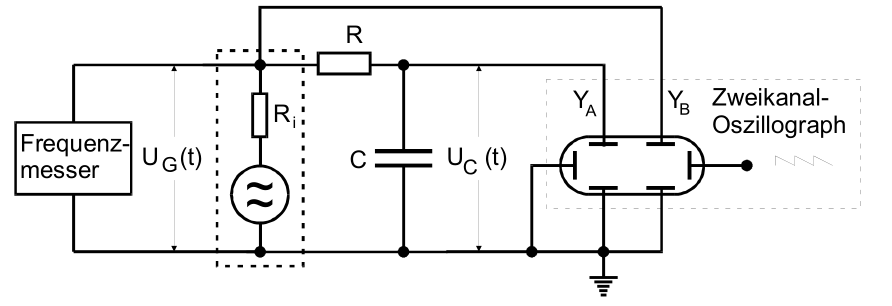
\includegraphics[width=0.7\textwidth]{latex/images/Phasenverschiebung.PNG}
            \caption{Schaltbild zur Bestimmung der Phasenverschiebung zwischen zwei Spannungen mit einem Zweikanal-Oszilloskop.\protect \cite{V353}.}
            \label{img:Phase}
        \end{figure}
        \noindent Messreihe c) untersucht die Phasenverschiebung zwischen Generatorspannung und Kondensatorspannung. Dazu wird die Schaltung aus 
        Abbildung(\ref{img:Phase}) genutzt. Für Phasen $\varphi > 0$ wird auf dem Schirm eine Bild wie in Abbildung(\ref{img:Zweist}) Dazu sehen sein.
        Aus diesem Bild ist dann der zeitliche Abstand a der beiden Nulldurchgänge und die Länge b abzulesen.



        \begin{figure}[H]
            \centering
            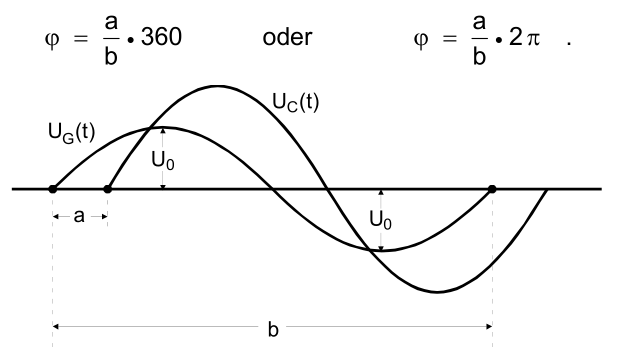
\includegraphics[width=0.5\textwidth]{latex/images/Zweistrahloszillograph.PNG}
            \caption{Messung der Phasenverschiebung zwischen zwei Spannungen mit dem Zweistrahloszillograph.\protect \cite{V353}.}
            \label{img:Zweist}
        \end{figure}

    \subsection{RC-Kreis als Integrator}

        \noindent Für diese Versuchsreihe wird wieder das Schaltbild aus Abbildung(\ref{img:Phase}) genutzt. Die anliegende Spannung wird auf 
        eine passende Frequenz eingestellt und dann der Reihe nach eine Rechteck-, Sinus und Dreiecksspannung angewandt. Nun wird der 
        integrierte und der zu integrierende Spannungsverlauf auf dem Bildschirm angezeigt und abgelesen.



        
        
